\documentclass[11pt]{article}

    \usepackage[breakable]{tcolorbox}
    \usepackage{parskip} % Stop auto-indenting (to mimic markdown behaviour)
    
    \usepackage{iftex}
    \ifPDFTeX
    	\usepackage[T1]{fontenc}
    	\usepackage{mathpazo}
    \else
    	\usepackage{fontspec}
    \fi

    % Basic figure setup, for now with no caption control since it's done
    % automatically by Pandoc (which extracts ![](path) syntax from Markdown).
    \usepackage{graphicx}
    % Maintain compatibility with old templates. Remove in nbconvert 6.0
    \let\Oldincludegraphics\includegraphics
    % Ensure that by default, figures have no caption (until we provide a
    % proper Figure object with a Caption API and a way to capture that
    % in the conversion process - todo).
    \usepackage{caption}
    \DeclareCaptionFormat{nocaption}{}
    \captionsetup{format=nocaption,aboveskip=0pt,belowskip=0pt}

    \usepackage[Export]{adjustbox} % Used to constrain images to a maximum size
    \adjustboxset{max size={0.9\linewidth}{0.9\paperheight}}
    \usepackage{float}
    \floatplacement{figure}{H} % forces figures to be placed at the correct location
    \usepackage{xcolor} % Allow colors to be defined
    \usepackage{enumerate} % Needed for markdown enumerations to work
    \usepackage{geometry} % Used to adjust the document margins
    \usepackage{amsmath} % Equations
    \usepackage{amssymb} % Equations
    \usepackage{textcomp} % defines textquotesingle
    % Hack from http://tex.stackexchange.com/a/47451/13684:
    \AtBeginDocument{%
        \def\PYZsq{\textquotesingle}% Upright quotes in Pygmentized code
    }
    \usepackage{upquote} % Upright quotes for verbatim code
    \usepackage{eurosym} % defines \euro
    \usepackage[mathletters]{ucs} % Extended unicode (utf-8) support
    \usepackage{fancyvrb} % verbatim replacement that allows latex
    \usepackage{grffile} % extends the file name processing of package graphics 
                         % to support a larger range
    \makeatletter % fix for grffile with XeLaTeX
    \def\Gread@@xetex#1{%
      \IfFileExists{"\Gin@base".bb}%
      {\Gread@eps{\Gin@base.bb}}%
      {\Gread@@xetex@aux#1}%
    }
    \makeatother

    % The hyperref package gives us a pdf with properly built
    % internal navigation ('pdf bookmarks' for the table of contents,
    % internal cross-reference links, web links for URLs, etc.)
    \usepackage{hyperref}
    % The default LaTeX title has an obnoxious amount of whitespace. By default,
    % titling removes some of it. It also provides customization options.
    \usepackage{titling}
    \usepackage{longtable} % longtable support required by pandoc >1.10
    \usepackage{booktabs}  % table support for pandoc > 1.12.2
    \usepackage[inline]{enumitem} % IRkernel/repr support (it uses the enumerate* environment)
    \usepackage[normalem]{ulem} % ulem is needed to support strikethroughs (\sout)
                                % normalem makes italics be italics, not underlines
    \usepackage{mathrsfs}
    

    
    % Colors for the hyperref package
    \definecolor{urlcolor}{rgb}{0,.145,.698}
    \definecolor{linkcolor}{rgb}{.71,0.21,0.01}
    \definecolor{citecolor}{rgb}{.12,.54,.11}

    % ANSI colors
    \definecolor{ansi-black}{HTML}{3E424D}
    \definecolor{ansi-black-intense}{HTML}{282C36}
    \definecolor{ansi-red}{HTML}{E75C58}
    \definecolor{ansi-red-intense}{HTML}{B22B31}
    \definecolor{ansi-green}{HTML}{00A250}
    \definecolor{ansi-green-intense}{HTML}{007427}
    \definecolor{ansi-yellow}{HTML}{DDB62B}
    \definecolor{ansi-yellow-intense}{HTML}{B27D12}
    \definecolor{ansi-blue}{HTML}{208FFB}
    \definecolor{ansi-blue-intense}{HTML}{0065CA}
    \definecolor{ansi-magenta}{HTML}{D160C4}
    \definecolor{ansi-magenta-intense}{HTML}{A03196}
    \definecolor{ansi-cyan}{HTML}{60C6C8}
    \definecolor{ansi-cyan-intense}{HTML}{258F8F}
    \definecolor{ansi-white}{HTML}{C5C1B4}
    \definecolor{ansi-white-intense}{HTML}{A1A6B2}
    \definecolor{ansi-default-inverse-fg}{HTML}{FFFFFF}
    \definecolor{ansi-default-inverse-bg}{HTML}{000000}

    % commands and environments needed by pandoc snippets
    % extracted from the output of `pandoc -s`
    \providecommand{\tightlist}{%
      \setlength{\itemsep}{0pt}\setlength{\parskip}{0pt}}
    \DefineVerbatimEnvironment{Highlighting}{Verbatim}{commandchars=\\\{\}}
    % Add ',fontsize=\small' for more characters per line
    \newenvironment{Shaded}{}{}
    \newcommand{\KeywordTok}[1]{\textcolor[rgb]{0.00,0.44,0.13}{\textbf{{#1}}}}
    \newcommand{\DataTypeTok}[1]{\textcolor[rgb]{0.56,0.13,0.00}{{#1}}}
    \newcommand{\DecValTok}[1]{\textcolor[rgb]{0.25,0.63,0.44}{{#1}}}
    \newcommand{\BaseNTok}[1]{\textcolor[rgb]{0.25,0.63,0.44}{{#1}}}
    \newcommand{\FloatTok}[1]{\textcolor[rgb]{0.25,0.63,0.44}{{#1}}}
    \newcommand{\CharTok}[1]{\textcolor[rgb]{0.25,0.44,0.63}{{#1}}}
    \newcommand{\StringTok}[1]{\textcolor[rgb]{0.25,0.44,0.63}{{#1}}}
    \newcommand{\CommentTok}[1]{\textcolor[rgb]{0.38,0.63,0.69}{\textit{{#1}}}}
    \newcommand{\OtherTok}[1]{\textcolor[rgb]{0.00,0.44,0.13}{{#1}}}
    \newcommand{\AlertTok}[1]{\textcolor[rgb]{1.00,0.00,0.00}{\textbf{{#1}}}}
    \newcommand{\FunctionTok}[1]{\textcolor[rgb]{0.02,0.16,0.49}{{#1}}}
    \newcommand{\RegionMarkerTok}[1]{{#1}}
    \newcommand{\ErrorTok}[1]{\textcolor[rgb]{1.00,0.00,0.00}{\textbf{{#1}}}}
    \newcommand{\NormalTok}[1]{{#1}}
    
    % Additional commands for more recent versions of Pandoc
    \newcommand{\ConstantTok}[1]{\textcolor[rgb]{0.53,0.00,0.00}{{#1}}}
    \newcommand{\SpecialCharTok}[1]{\textcolor[rgb]{0.25,0.44,0.63}{{#1}}}
    \newcommand{\VerbatimStringTok}[1]{\textcolor[rgb]{0.25,0.44,0.63}{{#1}}}
    \newcommand{\SpecialStringTok}[1]{\textcolor[rgb]{0.73,0.40,0.53}{{#1}}}
    \newcommand{\ImportTok}[1]{{#1}}
    \newcommand{\DocumentationTok}[1]{\textcolor[rgb]{0.73,0.13,0.13}{\textit{{#1}}}}
    \newcommand{\AnnotationTok}[1]{\textcolor[rgb]{0.38,0.63,0.69}{\textbf{\textit{{#1}}}}}
    \newcommand{\CommentVarTok}[1]{\textcolor[rgb]{0.38,0.63,0.69}{\textbf{\textit{{#1}}}}}
    \newcommand{\VariableTok}[1]{\textcolor[rgb]{0.10,0.09,0.49}{{#1}}}
    \newcommand{\ControlFlowTok}[1]{\textcolor[rgb]{0.00,0.44,0.13}{\textbf{{#1}}}}
    \newcommand{\OperatorTok}[1]{\textcolor[rgb]{0.40,0.40,0.40}{{#1}}}
    \newcommand{\BuiltInTok}[1]{{#1}}
    \newcommand{\ExtensionTok}[1]{{#1}}
    \newcommand{\PreprocessorTok}[1]{\textcolor[rgb]{0.74,0.48,0.00}{{#1}}}
    \newcommand{\AttributeTok}[1]{\textcolor[rgb]{0.49,0.56,0.16}{{#1}}}
    \newcommand{\InformationTok}[1]{\textcolor[rgb]{0.38,0.63,0.69}{\textbf{\textit{{#1}}}}}
    \newcommand{\WarningTok}[1]{\textcolor[rgb]{0.38,0.63,0.69}{\textbf{\textit{{#1}}}}}
    
    
    % Define a nice break command that doesn't care if a line doesn't already
    % exist.
    \def\br{\hspace*{\fill} \\* }
    % Math Jax compatibility definitions
    \def\gt{>}
    \def\lt{<}
    \let\Oldtex\TeX
    \let\Oldlatex\LaTeX
    \renewcommand{\TeX}{\textrm{\Oldtex}}
    \renewcommand{\LaTeX}{\textrm{\Oldlatex}}
    % Document parameters
    % Document title
    \title{Tarea1}
    \author{Benjamin Rivera}
    
    
    
    
    
% Pygments definitions
\makeatletter
\def\PY@reset{\let\PY@it=\relax \let\PY@bf=\relax%
    \let\PY@ul=\relax \let\PY@tc=\relax%
    \let\PY@bc=\relax \let\PY@ff=\relax}
\def\PY@tok#1{\csname PY@tok@#1\endcsname}
\def\PY@toks#1+{\ifx\relax#1\empty\else%
    \PY@tok{#1}\expandafter\PY@toks\fi}
\def\PY@do#1{\PY@bc{\PY@tc{\PY@ul{%
    \PY@it{\PY@bf{\PY@ff{#1}}}}}}}
\def\PY#1#2{\PY@reset\PY@toks#1+\relax+\PY@do{#2}}

\expandafter\def\csname PY@tok@w\endcsname{\def\PY@tc##1{\textcolor[rgb]{0.73,0.73,0.73}{##1}}}
\expandafter\def\csname PY@tok@c\endcsname{\let\PY@it=\textit\def\PY@tc##1{\textcolor[rgb]{0.25,0.50,0.50}{##1}}}
\expandafter\def\csname PY@tok@cp\endcsname{\def\PY@tc##1{\textcolor[rgb]{0.74,0.48,0.00}{##1}}}
\expandafter\def\csname PY@tok@k\endcsname{\let\PY@bf=\textbf\def\PY@tc##1{\textcolor[rgb]{0.00,0.50,0.00}{##1}}}
\expandafter\def\csname PY@tok@kp\endcsname{\def\PY@tc##1{\textcolor[rgb]{0.00,0.50,0.00}{##1}}}
\expandafter\def\csname PY@tok@kt\endcsname{\def\PY@tc##1{\textcolor[rgb]{0.69,0.00,0.25}{##1}}}
\expandafter\def\csname PY@tok@o\endcsname{\def\PY@tc##1{\textcolor[rgb]{0.40,0.40,0.40}{##1}}}
\expandafter\def\csname PY@tok@ow\endcsname{\let\PY@bf=\textbf\def\PY@tc##1{\textcolor[rgb]{0.67,0.13,1.00}{##1}}}
\expandafter\def\csname PY@tok@nb\endcsname{\def\PY@tc##1{\textcolor[rgb]{0.00,0.50,0.00}{##1}}}
\expandafter\def\csname PY@tok@nf\endcsname{\def\PY@tc##1{\textcolor[rgb]{0.00,0.00,1.00}{##1}}}
\expandafter\def\csname PY@tok@nc\endcsname{\let\PY@bf=\textbf\def\PY@tc##1{\textcolor[rgb]{0.00,0.00,1.00}{##1}}}
\expandafter\def\csname PY@tok@nn\endcsname{\let\PY@bf=\textbf\def\PY@tc##1{\textcolor[rgb]{0.00,0.00,1.00}{##1}}}
\expandafter\def\csname PY@tok@ne\endcsname{\let\PY@bf=\textbf\def\PY@tc##1{\textcolor[rgb]{0.82,0.25,0.23}{##1}}}
\expandafter\def\csname PY@tok@nv\endcsname{\def\PY@tc##1{\textcolor[rgb]{0.10,0.09,0.49}{##1}}}
\expandafter\def\csname PY@tok@no\endcsname{\def\PY@tc##1{\textcolor[rgb]{0.53,0.00,0.00}{##1}}}
\expandafter\def\csname PY@tok@nl\endcsname{\def\PY@tc##1{\textcolor[rgb]{0.63,0.63,0.00}{##1}}}
\expandafter\def\csname PY@tok@ni\endcsname{\let\PY@bf=\textbf\def\PY@tc##1{\textcolor[rgb]{0.60,0.60,0.60}{##1}}}
\expandafter\def\csname PY@tok@na\endcsname{\def\PY@tc##1{\textcolor[rgb]{0.49,0.56,0.16}{##1}}}
\expandafter\def\csname PY@tok@nt\endcsname{\let\PY@bf=\textbf\def\PY@tc##1{\textcolor[rgb]{0.00,0.50,0.00}{##1}}}
\expandafter\def\csname PY@tok@nd\endcsname{\def\PY@tc##1{\textcolor[rgb]{0.67,0.13,1.00}{##1}}}
\expandafter\def\csname PY@tok@s\endcsname{\def\PY@tc##1{\textcolor[rgb]{0.73,0.13,0.13}{##1}}}
\expandafter\def\csname PY@tok@sd\endcsname{\let\PY@it=\textit\def\PY@tc##1{\textcolor[rgb]{0.73,0.13,0.13}{##1}}}
\expandafter\def\csname PY@tok@si\endcsname{\let\PY@bf=\textbf\def\PY@tc##1{\textcolor[rgb]{0.73,0.40,0.53}{##1}}}
\expandafter\def\csname PY@tok@se\endcsname{\let\PY@bf=\textbf\def\PY@tc##1{\textcolor[rgb]{0.73,0.40,0.13}{##1}}}
\expandafter\def\csname PY@tok@sr\endcsname{\def\PY@tc##1{\textcolor[rgb]{0.73,0.40,0.53}{##1}}}
\expandafter\def\csname PY@tok@ss\endcsname{\def\PY@tc##1{\textcolor[rgb]{0.10,0.09,0.49}{##1}}}
\expandafter\def\csname PY@tok@sx\endcsname{\def\PY@tc##1{\textcolor[rgb]{0.00,0.50,0.00}{##1}}}
\expandafter\def\csname PY@tok@m\endcsname{\def\PY@tc##1{\textcolor[rgb]{0.40,0.40,0.40}{##1}}}
\expandafter\def\csname PY@tok@gh\endcsname{\let\PY@bf=\textbf\def\PY@tc##1{\textcolor[rgb]{0.00,0.00,0.50}{##1}}}
\expandafter\def\csname PY@tok@gu\endcsname{\let\PY@bf=\textbf\def\PY@tc##1{\textcolor[rgb]{0.50,0.00,0.50}{##1}}}
\expandafter\def\csname PY@tok@gd\endcsname{\def\PY@tc##1{\textcolor[rgb]{0.63,0.00,0.00}{##1}}}
\expandafter\def\csname PY@tok@gi\endcsname{\def\PY@tc##1{\textcolor[rgb]{0.00,0.63,0.00}{##1}}}
\expandafter\def\csname PY@tok@gr\endcsname{\def\PY@tc##1{\textcolor[rgb]{1.00,0.00,0.00}{##1}}}
\expandafter\def\csname PY@tok@ge\endcsname{\let\PY@it=\textit}
\expandafter\def\csname PY@tok@gs\endcsname{\let\PY@bf=\textbf}
\expandafter\def\csname PY@tok@gp\endcsname{\let\PY@bf=\textbf\def\PY@tc##1{\textcolor[rgb]{0.00,0.00,0.50}{##1}}}
\expandafter\def\csname PY@tok@go\endcsname{\def\PY@tc##1{\textcolor[rgb]{0.53,0.53,0.53}{##1}}}
\expandafter\def\csname PY@tok@gt\endcsname{\def\PY@tc##1{\textcolor[rgb]{0.00,0.27,0.87}{##1}}}
\expandafter\def\csname PY@tok@err\endcsname{\def\PY@bc##1{\setlength{\fboxsep}{0pt}\fcolorbox[rgb]{1.00,0.00,0.00}{1,1,1}{\strut ##1}}}
\expandafter\def\csname PY@tok@kc\endcsname{\let\PY@bf=\textbf\def\PY@tc##1{\textcolor[rgb]{0.00,0.50,0.00}{##1}}}
\expandafter\def\csname PY@tok@kd\endcsname{\let\PY@bf=\textbf\def\PY@tc##1{\textcolor[rgb]{0.00,0.50,0.00}{##1}}}
\expandafter\def\csname PY@tok@kn\endcsname{\let\PY@bf=\textbf\def\PY@tc##1{\textcolor[rgb]{0.00,0.50,0.00}{##1}}}
\expandafter\def\csname PY@tok@kr\endcsname{\let\PY@bf=\textbf\def\PY@tc##1{\textcolor[rgb]{0.00,0.50,0.00}{##1}}}
\expandafter\def\csname PY@tok@bp\endcsname{\def\PY@tc##1{\textcolor[rgb]{0.00,0.50,0.00}{##1}}}
\expandafter\def\csname PY@tok@fm\endcsname{\def\PY@tc##1{\textcolor[rgb]{0.00,0.00,1.00}{##1}}}
\expandafter\def\csname PY@tok@vc\endcsname{\def\PY@tc##1{\textcolor[rgb]{0.10,0.09,0.49}{##1}}}
\expandafter\def\csname PY@tok@vg\endcsname{\def\PY@tc##1{\textcolor[rgb]{0.10,0.09,0.49}{##1}}}
\expandafter\def\csname PY@tok@vi\endcsname{\def\PY@tc##1{\textcolor[rgb]{0.10,0.09,0.49}{##1}}}
\expandafter\def\csname PY@tok@vm\endcsname{\def\PY@tc##1{\textcolor[rgb]{0.10,0.09,0.49}{##1}}}
\expandafter\def\csname PY@tok@sa\endcsname{\def\PY@tc##1{\textcolor[rgb]{0.73,0.13,0.13}{##1}}}
\expandafter\def\csname PY@tok@sb\endcsname{\def\PY@tc##1{\textcolor[rgb]{0.73,0.13,0.13}{##1}}}
\expandafter\def\csname PY@tok@sc\endcsname{\def\PY@tc##1{\textcolor[rgb]{0.73,0.13,0.13}{##1}}}
\expandafter\def\csname PY@tok@dl\endcsname{\def\PY@tc##1{\textcolor[rgb]{0.73,0.13,0.13}{##1}}}
\expandafter\def\csname PY@tok@s2\endcsname{\def\PY@tc##1{\textcolor[rgb]{0.73,0.13,0.13}{##1}}}
\expandafter\def\csname PY@tok@sh\endcsname{\def\PY@tc##1{\textcolor[rgb]{0.73,0.13,0.13}{##1}}}
\expandafter\def\csname PY@tok@s1\endcsname{\def\PY@tc##1{\textcolor[rgb]{0.73,0.13,0.13}{##1}}}
\expandafter\def\csname PY@tok@mb\endcsname{\def\PY@tc##1{\textcolor[rgb]{0.40,0.40,0.40}{##1}}}
\expandafter\def\csname PY@tok@mf\endcsname{\def\PY@tc##1{\textcolor[rgb]{0.40,0.40,0.40}{##1}}}
\expandafter\def\csname PY@tok@mh\endcsname{\def\PY@tc##1{\textcolor[rgb]{0.40,0.40,0.40}{##1}}}
\expandafter\def\csname PY@tok@mi\endcsname{\def\PY@tc##1{\textcolor[rgb]{0.40,0.40,0.40}{##1}}}
\expandafter\def\csname PY@tok@il\endcsname{\def\PY@tc##1{\textcolor[rgb]{0.40,0.40,0.40}{##1}}}
\expandafter\def\csname PY@tok@mo\endcsname{\def\PY@tc##1{\textcolor[rgb]{0.40,0.40,0.40}{##1}}}
\expandafter\def\csname PY@tok@ch\endcsname{\let\PY@it=\textit\def\PY@tc##1{\textcolor[rgb]{0.25,0.50,0.50}{##1}}}
\expandafter\def\csname PY@tok@cm\endcsname{\let\PY@it=\textit\def\PY@tc##1{\textcolor[rgb]{0.25,0.50,0.50}{##1}}}
\expandafter\def\csname PY@tok@cpf\endcsname{\let\PY@it=\textit\def\PY@tc##1{\textcolor[rgb]{0.25,0.50,0.50}{##1}}}
\expandafter\def\csname PY@tok@c1\endcsname{\let\PY@it=\textit\def\PY@tc##1{\textcolor[rgb]{0.25,0.50,0.50}{##1}}}
\expandafter\def\csname PY@tok@cs\endcsname{\let\PY@it=\textit\def\PY@tc##1{\textcolor[rgb]{0.25,0.50,0.50}{##1}}}

\def\PYZbs{\char`\\}
\def\PYZus{\char`\_}
\def\PYZob{\char`\{}
\def\PYZcb{\char`\}}
\def\PYZca{\char`\^}
\def\PYZam{\char`\&}
\def\PYZlt{\char`\<}
\def\PYZgt{\char`\>}
\def\PYZsh{\char`\#}
\def\PYZpc{\char`\%}
\def\PYZdl{\char`\$}
\def\PYZhy{\char`\-}
\def\PYZsq{\char`\'}
\def\PYZdq{\char`\"}
\def\PYZti{\char`\~}
% for compatibility with earlier versions
\def\PYZat{@}
\def\PYZlb{[}
\def\PYZrb{]}
\makeatother


    % For linebreaks inside Verbatim environment from package fancyvrb. 
    \makeatletter
        \newbox\Wrappedcontinuationbox 
        \newbox\Wrappedvisiblespacebox 
        \newcommand*\Wrappedvisiblespace {\textcolor{red}{\textvisiblespace}} 
        \newcommand*\Wrappedcontinuationsymbol {\textcolor{red}{\llap{\tiny$\m@th\hookrightarrow$}}} 
        \newcommand*\Wrappedcontinuationindent {3ex } 
        \newcommand*\Wrappedafterbreak {\kern\Wrappedcontinuationindent\copy\Wrappedcontinuationbox} 
        % Take advantage of the already applied Pygments mark-up to insert 
        % potential linebreaks for TeX processing. 
        %        {, <, #, %, $, ' and ": go to next line. 
        %        _, }, ^, &, >, - and ~: stay at end of broken line. 
        % Use of \textquotesingle for straight quote. 
        \newcommand*\Wrappedbreaksatspecials {% 
            \def\PYGZus{\discretionary{\char`\_}{\Wrappedafterbreak}{\char`\_}}% 
            \def\PYGZob{\discretionary{}{\Wrappedafterbreak\char`\{}{\char`\{}}% 
            \def\PYGZcb{\discretionary{\char`\}}{\Wrappedafterbreak}{\char`\}}}% 
            \def\PYGZca{\discretionary{\char`\^}{\Wrappedafterbreak}{\char`\^}}% 
            \def\PYGZam{\discretionary{\char`\&}{\Wrappedafterbreak}{\char`\&}}% 
            \def\PYGZlt{\discretionary{}{\Wrappedafterbreak\char`\<}{\char`\<}}% 
            \def\PYGZgt{\discretionary{\char`\>}{\Wrappedafterbreak}{\char`\>}}% 
            \def\PYGZsh{\discretionary{}{\Wrappedafterbreak\char`\#}{\char`\#}}% 
            \def\PYGZpc{\discretionary{}{\Wrappedafterbreak\char`\%}{\char`\%}}% 
            \def\PYGZdl{\discretionary{}{\Wrappedafterbreak\char`\$}{\char`\$}}% 
            \def\PYGZhy{\discretionary{\char`\-}{\Wrappedafterbreak}{\char`\-}}% 
            \def\PYGZsq{\discretionary{}{\Wrappedafterbreak\textquotesingle}{\textquotesingle}}% 
            \def\PYGZdq{\discretionary{}{\Wrappedafterbreak\char`\"}{\char`\"}}% 
            \def\PYGZti{\discretionary{\char`\~}{\Wrappedafterbreak}{\char`\~}}% 
        } 
        % Some characters . , ; ? ! / are not pygmentized. 
        % This macro makes them "active" and they will insert potential linebreaks 
        \newcommand*\Wrappedbreaksatpunct {% 
            \lccode`\~`\.\lowercase{\def~}{\discretionary{\hbox{\char`\.}}{\Wrappedafterbreak}{\hbox{\char`\.}}}% 
            \lccode`\~`\,\lowercase{\def~}{\discretionary{\hbox{\char`\,}}{\Wrappedafterbreak}{\hbox{\char`\,}}}% 
            \lccode`\~`\;\lowercase{\def~}{\discretionary{\hbox{\char`\;}}{\Wrappedafterbreak}{\hbox{\char`\;}}}% 
            \lccode`\~`\:\lowercase{\def~}{\discretionary{\hbox{\char`\:}}{\Wrappedafterbreak}{\hbox{\char`\:}}}% 
            \lccode`\~`\?\lowercase{\def~}{\discretionary{\hbox{\char`\?}}{\Wrappedafterbreak}{\hbox{\char`\?}}}% 
            \lccode`\~`\!\lowercase{\def~}{\discretionary{\hbox{\char`\!}}{\Wrappedafterbreak}{\hbox{\char`\!}}}% 
            \lccode`\~`\/\lowercase{\def~}{\discretionary{\hbox{\char`\/}}{\Wrappedafterbreak}{\hbox{\char`\/}}}% 
            \catcode`\.\active
            \catcode`\,\active 
            \catcode`\;\active
            \catcode`\:\active
            \catcode`\?\active
            \catcode`\!\active
            \catcode`\/\active 
            \lccode`\~`\~ 	
        }
    \makeatother

    \let\OriginalVerbatim=\Verbatim
    \makeatletter
    \renewcommand{\Verbatim}[1][1]{%
        %\parskip\z@skip
        \sbox\Wrappedcontinuationbox {\Wrappedcontinuationsymbol}%
        \sbox\Wrappedvisiblespacebox {\FV@SetupFont\Wrappedvisiblespace}%
        \def\FancyVerbFormatLine ##1{\hsize\linewidth
            \vtop{\raggedright\hyphenpenalty\z@\exhyphenpenalty\z@
                \doublehyphendemerits\z@\finalhyphendemerits\z@
                \strut ##1\strut}%
        }%
        % If the linebreak is at a space, the latter will be displayed as visible
        % space at end of first line, and a continuation symbol starts next line.
        % Stretch/shrink are however usually zero for typewriter font.
        \def\FV@Space {%
            \nobreak\hskip\z@ plus\fontdimen3\font minus\fontdimen4\font
            \discretionary{\copy\Wrappedvisiblespacebox}{\Wrappedafterbreak}
            {\kern\fontdimen2\font}%
        }%
        
        % Allow breaks at special characters using \PYG... macros.
        \Wrappedbreaksatspecials
        % Breaks at punctuation characters . , ; ? ! and / need catcode=\active 	
        \OriginalVerbatim[#1,codes*=\Wrappedbreaksatpunct]%
    }
    \makeatother

    % Exact colors from NB
    \definecolor{incolor}{HTML}{303F9F}
    \definecolor{outcolor}{HTML}{D84315}
    \definecolor{cellborder}{HTML}{CFCFCF}
    \definecolor{cellbackground}{HTML}{F7F7F7}
    
    % prompt
    \makeatletter
    \newcommand{\boxspacing}{\kern\kvtcb@left@rule\kern\kvtcb@boxsep}
    \makeatother
    \newcommand{\prompt}[4]{
        \ttfamily\llap{{\color{#2}[#3]:\hspace{3pt}#4}}\vspace{-\baselineskip}
    }
    

    
    % Prevent overflowing lines due to hard-to-break entities
    \sloppy 
    % Setup hyperref package
    \hypersetup{
      breaklinks=true,  % so long urls are correctly broken across lines
      colorlinks=true,
      urlcolor=urlcolor,
      linkcolor=linkcolor,
      citecolor=citecolor,
      }
    % Slightly bigger margins than the latex defaults
    
    \usepackage[spanish]{babel}
    \geometry{verbose,tmargin=0.7in,bmargin=0.7in,lmargin=0.5in,rmargin=2.4in}
    
    

\begin{document}
    
    \maketitle
    \tableofcontents    

    
    \hypertarget{tarea-1}{%
\part*{Tarea 1}\label{tarea-1}}

\emph{Tarea 1} de \emph{Benjamín Rivera} para el curso de
\textbf{Métodos Numéricos} impartido por \emph{Joaquín Peña Acevedo}.
Fecha limite de entrega \textbf{6 de Septiembre de 2020}.

\newpage
    \hypertarget{como-ejecutar}{%
\section*{Como ejecutar}\label{como-ejecutar}}

    \hypertarget{requerimientos}{%
\paragraph{Requerimientos}\label{requerimientos}}

Este programa se ejecuto en mi computadora con la version de
\textbf{Python 3.8.2} y con estos
\href{https://github.com/BenchHPZ/UG-Compu/blob/master/MN/requerimientos.txt}{requerimientos}

\hypertarget{jupyter}{%
\subsection*{Jupyter}\label{jupyter}}

En caso de tener acceso a un \emph{servidor jupyter} ,con los
requerimientos antes mencionados, unicamente basta con ejecutar todas
las celdas de este \emph{notebook}. Probablemente no todas las celdas de
\emph{markdown} produzcan el mismo resultado por las
\href{jupyter-contrib-nbextensions.readthedocs.io}{\emph{Nbextensions}}.

\hypertarget{consola}{%
\subsection*{Consola}\label{consola}}

Habrá archivos e instrucciones para poder ejecutar cada uno de los
ejercicios desde la consola.

\hypertarget{si-todo-sale-mal}{%
\subsection*{Si todo sale mal}\label{si-todo-sale-mal}}

En caso de que todo salga mal, tratare de dejar una copia disponible en
\textbf{GoogleColab} que se pueda ejecutar con la versión de
\textbf{Python} de \emph{GoogleColab}


\newpage
    \hypertarget{ejercicio-1}{%
\section{Ejercicio 1}\label{ejercicio-1}}

Supongamos que una computadora tiene 8 dígitos para representar la parte
fraccionaria de un número de punto flotante.

    \hypertarget{calcular-el-valor-del-uxe9psilon-de-la-muxe1quina}{%
\subsection{Calcular el valor del épsilon de la
máquina}\label{calcular-el-valor-del-uxe9psilon-de-la-muxe1quina}}

    En clase vimos que si conocemos la cantidad de bits \(p\) para
representar la parte fraccionaria de la mantisa, entonces

\begin{equation} \epsilon_m = (1.0)_2 \times 2^{-p} \label{eq:epsilon}\end{equation}

Dado que sabemos que la máquina de este ejercicio usara \(8bits\) para
representar la parte fraccionaria entonces, por \ref{eq:epsilon}, el
\(\epsilon_m\) para este ejercicio es

\begin{equation*} \epsilon_m = (1.0)_2 \times 2^{-8} = 3.90625 \times 10^{-3}
\label{eq:epsilon maquina} \end{equation*}

    \begin{tcolorbox}[breakable, size=fbox, boxrule=1pt, pad at break*=1mm,colback=cellbackground, colframe=cellborder]
\prompt{In}{incolor}{1}{\boxspacing}
\begin{Verbatim}[commandchars=\\\{\}]
\PY{n+nb}{print}\PY{p}{(}\PY{l+m+mi}{2}\PY{o}{*}\PY{o}{*}\PY{p}{(}\PY{o}{\PYZhy{}}\PY{l+m+mi}{8}\PY{p}{)}\PY{p}{)}
\end{Verbatim}
\end{tcolorbox}

    \begin{Verbatim}[commandchars=\\\{\}]
0.00390625
    \end{Verbatim}

    \hypertarget{dar-la-representaciuxf3n-en-notaciuxf3n-cientifica-mantisa-base-2-multiplicada-por-2-elevda-al-exponente-correspondiente-del-nuxfamero-5.}{%
\subsection{Dar la representación en notación cientifica (mantisa
base 2, multiplicada por 2 elevda al exponente correspondiente) del
número
5.}\label{dar-la-representaciuxf3n-en-notaciuxf3n-cientifica-mantisa-base-2-multiplicada-por-2-elevda-al-exponente-correspondiente-del-nuxfamero-5.}}

    Sabemos que el número \(5\) se representa en binario como \((101)_2\).
Como los números se prefieren normalizados entonces debemos representar
\((1.01)_2\) en la notación solicitada. Por lo que

\begin{equation*} 5 = (101)_2 \times 2^0 = (1.01)_2 \times 2^2 = 1.25 \times 2^2
\end{equation*}

    \hypertarget{dar-la-representaciuxf3n-cientuxedfica-del-nuxfamero-consecutico-a-5-en-la-computadora.-escribir-la-distancia-d_c-entre-5-y-su-consecutivo.-expresar-d_c-en-tuxe9rminos-del-uxe9pslon-de-la-muxe1quina.}{%
\subsection{\texorpdfstring{Dar la representación científica del
número consecutico a 5 en la computadora. Escribir la distancia \(d_c\)
entre 5 y su consecutivo. Expresar \(d_c\) en términos del épslon de la
máquina.}{Dar la representación científica del número consecutico a 5 en la computadora. Escribir la distancia d\_c entre 5 y su consecutivo. Expresar d\_c en términos del épslon de la máquina.}}\label{dar-la-representaciuxf3n-cientuxedfica-del-nuxfamero-consecutico-a-5-en-la-computadora.-escribir-la-distancia-d_c-entre-5-y-su-consecutivo.-expresar-d_c-en-tuxe9rminos-del-uxe9pslon-de-la-muxe1quina.}}

    Sabemos que el número consecutivo \((5_c)\) a \(5\) en esta computadora
es \(5+\epsilon_m\). Si extendemos toda la mantisa de \(5\) este se ve
\((1.01000000)\). Y sumar \(\epsilon_m\) implica sumar \(1\) a la
mantisa, enspecificamente en esta computadora, al \(bit 8\) de la
mantisa. De manera que

\begin{eqnarray*} 
    5_c &=& 5 + \epsilon_m 
    = (1.01)_2 \times 2^2 + (1.0)_2 \times 2^{2-8} \\ 
    &=& ((1.01000000)_2 + (0.00000001)_2) \times 2^2 \\
    &=& (1.01000001)_2 \times 2^2 \\
    &=& 5.015625
\end{eqnarray*}

por lo que la distancia entre \(5\) y su consecutivo \(5+\epsilon_m\) es

\begin{equation*} d_c = (5+\epsilon_m)-5 = \epsilon_m \times 2^2 = (0.00000001)_2 \times 2^2 = 0.015625
\end{equation*}

    \hypertarget{tenemos-que-el-consecutivo-de-5-es-expresable-como-5-d_c.-si-tenemos-un-x-real-tal-que-x-in-5-5d_c-entonces-la-computadora-representara-a-x-como-flx5-o-flx5d_c.-escribir-una-cota-para-el-error-relativo-para-las-dos-posibles-represetnaciones-de-x}{%
\subsection{\texorpdfstring{Tenemos que el consecutivo de \(5\) es
expresable como \(5 + d_c\). Si tenemos un \(x\) real tal que
\(x \in (5, 5+d_c)\) entonces la computadora representara a \(x\) como
\(fl(x)=5\) o \(fl(x)=5+d_c\). Escribir una cota para el error relativo
para las dos posibles represetnaciones de
x}{Tenemos que el consecutivo de 5 es expresable como 5 + d\_c. Si tenemos un x real tal que x \textbackslash{}in (5, 5+d\_c) entonces la computadora representara a x como fl(x)=5 o fl(x)=5+d\_c. Escribir una cota para el error relativo para las dos posibles represetnaciones de x}}\label{tenemos-que-el-consecutivo-de-5-es-expresable-como-5-d_c.-si-tenemos-un-x-real-tal-que-x-in-5-5d_c-entonces-la-computadora-representara-a-x-como-flx5-o-flx5d_c.-escribir-una-cota-para-el-error-relativo-para-las-dos-posibles-represetnaciones-de-x}}

    \begin{quote}
Error relativo \begin{equation*}
\left| \frac{fl(x) - x}{x} \right|
\end{equation*}
\end{quote}

Sabemos que las dos posibles representaciones son el \emph{truncamiento}
y el \emph{redondeo} ,para dar la cota se deben calcular los valores
minimos y maximos del error relativo. En general trabajaremos con

\begin{equation} \label{eq:error relativo}
    \left| \frac{fl(x) - x}{x} \right| = \left| \frac{fl(x)}{x} - 1 \right| 
\end{equation}

Antes de continuar es importante notar lo siguiente. Sabemos que, para
ambos casos, el dominio de la función sera \([5, 5+d_c]\). Además,
notemos que el rango de \(\frac{fl(x)}{x}\), para nuestro dominio y los
dos valores que puede tomar \(fl(x)\), es
\(\left[ \frac{5}{5+d_c}, \frac{5+d_c}{5} \right]\). Por ultimo, sabemos
que \(\frac{fl(x)}{x}\) es descendente para \(x>0\).

    \textbf{Truncamiento} Para el truncamiento \(fl(x) = 5\) por lo que
debemos calcular la cota para

\begin{equation*} Er_\_ = \left| \frac{5}{x} - 1 \right|
\end{equation*}

En este caso, el rango de \(\frac{fl(x)}{x} = \frac{5}{x}\) es
\(\left[ \frac{5}{5+d_c}, \frac{5}{5}=1 \right]\) por lo que el rango de
\(Er_\_\) es \(\left[ 0, |\frac{5}{5+d_c}-1| \right]\). Por iluminación
divina, suponemos que esta función es ascendente, y por lo tanto
\(Er_\_(5) < Er_\_(5+dc)\). Primero evaluamos la función en estos puntos

\begin{equation*} Er_\_(5) = \left|\frac{5}{5} -1\right| = 0 \quad\quad Er_\_(5+d_c) = \left|\frac{5}{5+d_c} -1 \right| \sim 0.00311
\end{equation*}

Por lo que, usando el truncamiento, esta \textbf{función esta acotada}
por \(\left[ Er_\_(5), Er_\_(5+d_c) \right]\)

    \textbf{Redondeo} Procedemos de manera similar al anterior. Para el
redondeo tenemos que \(fl(x) = 5+d_c\), esto nos da la expresion

\begin{equation*} Er_+ = \left| \frac{5+d_c}{x} - 1 \right|
\end{equation*}

Y de manera similar al anterior podemos ver que esta función es
descendente, por lo que \(Er_+(5+d_c) < Er_+(d_c)\)

\begin{equation*} Er_+(5+d_c) = \left| \frac{5+d_c}{5+d_c} -1 \right| = 0 \quad\quad Er_+(5) = \left| \frac{5+d_c}{5} -1 \right| \sim 0.00312
\end{equation*}

De manera que esta función queda acotada por
\(\left[ Er_+(5+d_c),Er_+(5) \right]\)

    \hypertarget{explique-si-los-siguientes-nuxfameros-tienen-respresentaciuxf3n-exacta-en-la-computadora-es-decir-si-fla_ia_i}{%
\subsection{\texorpdfstring{Explique si los siguientes números tienen
respresentación exacta en la computadora, es decir, si
\(fl(a_i)=a_i\)}{Explique si los siguientes números tienen respresentación exacta en la computadora, es decir, si fl(a\_i)=a\_i}}\label{explique-si-los-siguientes-nuxfameros-tienen-respresentaciuxf3n-exacta-en-la-computadora-es-decir-si-fla_ia_i}}

    \begin{itemize}
\tightlist
\item
  \(a_1 = \epsilon/2\)

  \par

  Sabemos que en el sistema de este ejercicio (\(8bits\) parte flotante)
  \(\epsilon_m = (1.0)_2 \times 2^{-8}\), de manera que,
\end{itemize}

\begin{equation*} \epsilon_m/2 = \frac{(1.0)_2 \times 2^{-8}}{2} = (1.0)_2 \times 2^{-9}
 \end{equation*}

por lo que, mientras que el rango del exponente sea suficiente (dado que
el ejercicio solo da información del tamaño de la \textit{matisa}), este
número \textbf{es representable} en el sistema.

\begin{itemize}
\tightlist
\item
  \(a_2 = 1+ \epsilon/2\)

  \par

  De manera que \(a_2\) se expresa como
\end{itemize}

\begin{equation*} a_2 = (1.0)_2 + \epsilon/2 = (1.0)_2 + (1.0)_2 \times 2^{-9} = (1.000000001)_2
 \end{equation*}

pero como este sistema solo usa \(8bits\) para la mantisa entonces, para
este sistema

\begin{equation*} a_2 = (1.0)_2 + \epsilon/2 = (1.000000001)_2 = (1.0)_2
 \end{equation*}

por lo que este número \textbf{no tiene representación} en este sistema.

\begin{itemize}
\tightlist
\item
  \(a_3 = 1- \epsilon\)

  \par

  Este número se escribe como
\end{itemize}

\begin{eqnarray*} 
     a_3 = 1- \epsilon &=& (1.0)_2 - (1.0)_2 \times 2^{-8} \\
         &=& (1.00000000)_2 - (0.00000001)_2 \\
         &=& (0.11111111)_2 \\
         &=& (1.1111111)_2 \times 2^{-1}
 \end{eqnarray*}

por lo que este número \textbf{si tiene una representación} en este
sistema.

\begin{itemize}
\tightlist
\item
  \(a_4 = 1- \epsilon/2\)

  \par

  Como con los anteriores, esta operación se expresa como
\end{itemize}

\begin{eqnarray*}
     a_4 = 1- \epsilon/2 &=& (1.0)_2 - (1.0)_2 \times 2^{-9} \\
         &=& (1.00000000)_2 - (0.000000001)_2 \\
         &=& (0.111111111)_2 \\
         &=& (1.11111111)_2 \times 2^{-1}
 \end{eqnarray*}

el cual \textbf{si tiene respresentación} en el sistema de este
ejercicio.

\begin{itemize}
\tightlist
\item
  \(a_5 = 1- \epsilon/4\)

  \par

  En este inciso primero calcularemos \(\epsilon/4\), para el cual
  expandimos lo siguiente
\end{itemize}

\begin{equation*} \epsilon/4 = \frac{(1.0)_2 \times 2^{-8}}{2^2} = (1.0)_2 \times 2^{-10}
 \end{equation*}

el cual, mientras el exponente alcance, \emph{si es representable} en el
sistema. Por otro lado, el numero de este inciso nos da

\begin{eqnarray*}
     a_5 = 1 - \epsilon/4 &=& (1.0)_2 - (1.0)_2 \times 2^{-10} \\
         &=& (1.00000000)_2 - (0.0000000001)_2 \\
         &=& (0.1111111111)_2 \\
         &=& (1.111111111)_2 \times 2^{-1}
 \end{eqnarray*}

pero este número tiene una mantisa de \(9bits\), por lo cual, \textbf{no
tiene representación} en el sistema.

\begin{itemize}
\tightlist
\item
  \(a_6 = \epsilon^2\)

  \par

  Para este inciso
\end{itemize}

\begin{equation} a_6 = \epsilon^2 = ((1.0)_2 \times 2^{-8})_2^2 = (1.0)_2 \times 2^{-16} 
 \end{equation}

el cual \textbf{si tiene represetación} en el sistema.

\begin{itemize}
\tightlist
\item
  \(a_7 = 0.125\)

  \par

  Primero pasamos de el número de decimal a binario, de manera que
  \((0.125)_{10} = (0.001)_{2}\). Luego hay que normalizarlo, por lo que
  \((0.001)_{2} = (1.0)_{2} \times 2^{-3}\). Por lo que este numero
  \textbf{si tiene respresentacion} en el sistema.
\item
  \(a_8 = 2^{-10}\)

  \par

  Y por 'ultimo, tenemos que
\end{itemize}

\begin{equation*} a_8 = 2^{-10} = ((10.0)_2)^{-10} = ((1.0)_2 \times 2^{1})^{-10} = (1.0)_2 \times 2^{-10}
 \end{equation*}

    \hypertarget{de-una-cota-para-el-error-relativo-de-las-restas-y-respecto-al-verdader-valor.-suponga-que-flx-se-obtiene-por-redondeo-hacia-abajo-truncamiento}{%
\subsection{\texorpdfstring{De una cota para el error relativo de las
restas \ref{eq:resta 1} y \ref{eq:resta 2} respecto al verdader valor.
Suponga que \(fl(x)\) se obtiene por redondeo hacia abajo
\emph{(truncamiento)}}{De una cota para el error relativo de las restas  y  respecto al verdader valor. Suponga que fl(x) se obtiene por redondeo hacia abajo (truncamiento)}}\label{de-una-cota-para-el-error-relativo-de-las-restas-y-respecto-al-verdader-valor.-suponga-que-flx-se-obtiene-por-redondeo-hacia-abajo-truncamiento}}

    \begin{equation}
    fl(0.9) - fl(0.5)   \label{eq:resta 1}
\end{equation} \begin{equation}
    fl(0.9) - fl(0.895) \label{eq:resta 2}
\end{equation}

Para este ejercicio, dado que nos pide usar el \textit{truncamiento},
definimos a la \textbf{unidad de redondeo} como \(u = \epsilon_m/2\).
Esto tambien nos define a \(fl(x)=x(1+\delta)\) y \(|\delta| \leq u\).
Adem'as, siguiendo las notas, podemos usar la cota que ah'i se
proporciona y sustituir \(u\).

\begin{equation} |\delta_{x-y}| \leq \frac{\epsilon}{2}\frac{|x|+|y|}{|x-y|} \label{eq:cota}
\end{equation}

Y antes de continuar calculamos \(\epsilon_m/2\) para poder usarlo mas
adelante. De manera que

\begin{equation*} \epsilon_m/2 = \frac{(1.0)_2 \times 2^{-8}}{2} = (1.0)_2 \times 2^{-9}
\end{equation*}

Y, como tambien lo usaremos, es bueno tener en cuenta.

\begin{equation*} \delta_{x-y} = \frac{fl(x)-fl(y) - (x-y)}{x-y}
\end{equation*}

    Empezamos por la operaci'on \ref{eq:resta 1}, de donde obtenemos
\(x=0.9\) y \(y=0.5\). Primero calculamos los valores de maquina de
estos. \begin{eqnarray*}
     fl(x) = fl(0.9) &=& (1.1100(1100))_2\times 2^{-1} \\
             &=& (1.11001100)_2\times 2^{-1}  \quad\quad\quad \text{(Truncamiento (no cabe))} \\
             &\sim& 0.8984375
            \\ & & \\ & & \\
     fl(y) = fl(0.5) &=& (1.0)_2\times 2^{-1} \\
             &=& (1.00000000)_2\times 2^{-1}  \quad\quad\quad \text{(Truncamiento (si cabe))} \\
             &=& 0.5
 \end{eqnarray*}

De manera que, como ya conocemos \(\epsilon_m\), los valores de la
operaci'on y sus representaciones en el sistema, procedemos a encontrar
la cota. Dado que usamos la cota de las notas, unicamente queda
sustituir, de esto obtenemos que:

\begin{eqnarray*}
    \delta_{x-y} \sim -0.00390625 \\
    \frac{\epsilon}{2}\frac{|x|+|y|}{|x-y|} = 0.00683593
\end{eqnarray*}

Por lo que, siguiendo la cota de la ecuaci'on \ref{eq:cota}, podemos
decir que esta operaci'on esta acotada por

\begin{equation*}
    |\delta_{x-y}| \sim 0.00390625 \leq 0.00683593 \sim \frac{\epsilon}{2}\frac{|x|+|y|}{|x-y|}
\end{equation*}

    De manera similar, para la operaci'on \ref{eq:resta 2}, tenemos que
\(x=0.9\) y \(y=0.895\). Calculamos los redondondeos de la computadora.

\begin{eqnarray*}
     fl(x) = fl(0.9) &=& (1.1100(1100))_2\times 2^{-1} \\
             &=& (1.11001100)_2\times 2^{-1}  \quad\quad\quad \text{(Truncamiento (no cabe))} \\
             &\sim& 0.8984375
             \\&&\\&&\\
     fl(y) = fl(0.895) &=& (1.1100101000111101)_2\times 2^{-1} \\
             &=& (1.11001010)_2\times 2^{-1}  \quad\quad\quad \text{(Truncamiento (no cabe))} \\
             &=& 0.89453125
 \end{eqnarray*}

Ahora procedemos a calcular los limites de la cota, por lo que

\begin{eqnarray*}
    \delta_{x-y} \sim  -0.21875\\
    \frac{\epsilon}{2}\frac{|x|+|y|}{|x-y|} = 0.70117187
\end{eqnarray*}

Y por 'ultimo, seg'un la cota \ref{eq:cota}, acotamos esta operaci'on
por

\begin{equation*}
    |\delta_{x-y}| \sim -0.21875 \leq 0.70117187 \sim \frac{\epsilon}{2}\frac{|x|+|y|}{|x-y|}
\end{equation*}

\newpage
    \hypertarget{ejercicio-2}{%
\section{Ejercicio 2}\label{ejercicio-2}}

    Programe la función \texttt{epsilonFloat} que devuelve el épsilon de la
máquina \(\epsilon_m\) para números de simple precisión y la función
\texttt{epsilonDouble} para números de doble precisión.

\begin{verbatim}
epsilon = 1.0
unidad = 1.0
valor = unidad + epsilon
while valor > unidad
    epsilon = epsilon/2
    valor = end + epsilon
end while
epsilon = epsilon*2
\end{verbatim}

Usar el algoritmo visto en clase.

    \begin{tcolorbox}[breakable, size=fbox, boxrule=1pt, pad at break*=1mm,colback=cellbackground, colframe=cellborder]
\prompt{In}{incolor}{3}{\boxspacing}
\begin{Verbatim}[commandchars=\\\{\}]
\PY{c+c1}{\PYZsh{} Primera parte del ejercicio 1}
\PY{k+kn}{import} \PY{n+nn}{numpy} \PY{k}{as} \PY{n+nn}{np}

\PY{k}{def} \PY{n+nf}{epsilonMaquina}\PY{p}{(}\PY{n}{tipoDato}\PY{p}{)}\PY{p}{:}
    \PY{l+s+sd}{\PYZdq{}\PYZdq{}\PYZdq{} Funcion que trata de calcular el epsilon }
\PY{l+s+sd}{    de la maquina mediante el algoritmo antes pre\PYZus{}}
\PY{l+s+sd}{    sentado. }
\PY{l+s+sd}{    Input:}
\PY{l+s+sd}{        tipoDato := esta pensado para ser uno de }
\PY{l+s+sd}{            los tipos proporcionados por la li\PYZus{}}
\PY{l+s+sd}{            breria numpy.}
\PY{l+s+sd}{    Output:}
\PY{l+s+sd}{        Regresa el epsilon de la maquina calcula\PYZus{}}
\PY{l+s+sd}{            do con el tipo de dato especificado.}
\PY{l+s+sd}{    \PYZdq{}\PYZdq{}\PYZdq{}}
    \PY{k}{return} \PY{n}{epsilon}\PY{o}{*}\PY{l+m+mi}{2}

\PY{k}{def} \PY{n+nf}{epsilonFloat}\PY{p}{(}\PY{p}{)}\PY{p}{:}
    \PY{l+s+sd}{\PYZdq{}\PYZdq{}\PYZdq{} Calculamos el epsilon de la maquina con }
\PY{l+s+sd}{    precision de 32bits}
\PY{l+s+sd}{    \PYZdq{}\PYZdq{}\PYZdq{}}
    \PY{k}{return} \PY{n}{epsilonMaquina}\PY{p}{(}\PY{n}{np}\PY{o}{.}\PY{n}{float32}\PY{p}{)}

\PY{k}{def} \PY{n+nf}{epsilonDouble}\PY{p}{(}\PY{p}{)}\PY{p}{:}
    \PY{l+s+sd}{\PYZdq{}\PYZdq{}\PYZdq{} Calculamos el epsilon de la maquina con}
\PY{l+s+sd}{    precision de 64 bits}
\PY{l+s+sd}{        A pesar de que el flotante de python ya}
\PY{l+s+sd}{    tiene esta precision, creo que es convenien\PYZus{}}
\PY{l+s+sd}{    te especificarlo.}
\PY{l+s+sd}{    \PYZdq{}\PYZdq{}\PYZdq{}}
    \PY{k}{return} \PY{n}{epsilonMaquina}\PY{p}{(}\PY{n}{np}\PY{o}{.}\PY{n}{float64}\PY{p}{)}

\PY{c+c1}{\PYZsh{} Epsilons calculados}

\PY{n}{eF} \PY{o}{=} \PY{n}{np}\PY{o}{.}\PY{n}{float32}\PY{p}{(}\PY{n}{epsilonFloat}\PY{p}{(}\PY{p}{)}\PY{p}{)}
\PY{n}{eD} \PY{o}{=} \PY{n}{np}\PY{o}{.}\PY{n}{float64}\PY{p}{(}\PY{n}{epsilonDouble}\PY{p}{(}\PY{p}{)}\PY{p}{)}

\PY{c+c1}{\PYZsh{} Imprimir en pantalla}
\PY{n+nb}{print}\PY{p}{(}\PY{l+s+sa}{...}\PY{p}{)}
\end{Verbatim}
\end{tcolorbox}

    \begin{Verbatim}[commandchars=\\\{\}]
Se calculalron los epsilons
        eF=1.1920929e-07 y
        eD=2.220446049250313e-16
para 32 y 64 bits correspondientemente.

    \end{Verbatim}

    \begin{tcolorbox}[breakable, size=fbox, boxrule=1pt, pad at break*=1mm,colback=cellbackground, colframe=cellborder]
\prompt{In}{incolor}{4}{\boxspacing}
\begin{Verbatim}[commandchars=\\\{\}]
\PY{c+c1}{\PYZsh{} Segunda parte del ejercicio 1}
\PY{k}{def} \PY{n+nf}{respuesta}\PY{p}{(}\PY{n}{res}\PY{p}{)}\PY{p}{:}
    \PY{l+s+sd}{\PYZdq{}\PYZdq{}\PYZdq{} Funcion para formatear la respuesta. \PYZdq{}\PYZdq{}\PYZdq{}}
    \PY{k}{return} \PY{l+s+s2}{\PYZdq{}}\PY{l+s+s2}{iguales}\PY{l+s+s2}{\PYZdq{}} \PY{k}{if} \PY{n}{res} \PY{k}{else} \PY{l+s+s2}{\PYZdq{}}\PY{l+s+s2}{diferentes}\PY{l+s+s2}{\PYZdq{}}
\PY{k}{def} \PY{n+nf}{comparacion}\PY{p}{(}\PY{n}{epsilon}\PY{p}{)}\PY{p}{:}
    \PY{l+s+sd}{\PYZdq{}\PYZdq{}\PYZdq{} Esta funcion resivira el epsilon a eva\PYZus{}}
\PY{l+s+sd}{    luar y el tipo de dato al que este correspon\PYZus{}}
\PY{l+s+sd}{    de para hacer las comparaciones solicitadas}
\PY{l+s+sd}{    en el ejercicio.}
\PY{l+s+sd}{    Input:}
\PY{l+s+sd}{        epsilon a considerar en la comparacion }
\PY{l+s+sd}{    Output:}
\PY{l+s+sd}{        Las respuestas son procesadas por la}
\PY{l+s+sd}{        funcion respuesta para obtener el for\PYZus{}}
\PY{l+s+sd}{        mato solicitado}
\PY{l+s+sd}{    \PYZdq{}\PYZdq{}\PYZdq{}}
    \PY{c+c1}{\PYZsh{} Comprobaciones}
    \PY{n+nb}{print}\PY{p}{(}\PY{l+s+sa}{f}\PY{l+s+s1}{\PYZsq{}}\PY{l+s+si}{\PYZob{}}\PY{n}{respuesta}\PY{p}{(} \PY{n}{tD}\PY{p}{(}\PY{l+m+mi}{1} \PY{o}{+} \PY{n}{epsilon} \PY{p}{)}   \PY{o}{==} \PY{l+m+mi}{1} \PY{p}{)}  \PY{l+s+si}{=\PYZcb{}}\PY{l+s+s1}{\PYZsq{}}\PY{p}{)}
    \PY{n+nb}{print}\PY{p}{(}\PY{l+s+sa}{f}\PY{l+s+s1}{\PYZsq{}}\PY{l+s+si}{\PYZob{}}\PY{n}{respuesta}\PY{p}{(} \PY{n}{tD}\PY{p}{(} \PY{n}{epsilon}\PY{o}{/}\PY{l+m+mi}{2} \PY{p}{)}    \PY{o}{==} \PY{l+m+mi}{0} \PY{p}{)}  \PY{l+s+si}{=\PYZcb{}}\PY{l+s+s1}{\PYZsq{}}\PY{p}{)}
    \PY{n+nb}{print}\PY{p}{(}\PY{l+s+sa}{f}\PY{l+s+s1}{\PYZsq{}}\PY{l+s+si}{\PYZob{}}\PY{n}{respuesta}\PY{p}{(} \PY{n}{tD}\PY{p}{(}\PY{l+m+mi}{1} \PY{o}{+} \PY{n}{epsilon}\PY{o}{/}\PY{l+m+mi}{2} \PY{p}{)} \PY{o}{==} \PY{l+m+mi}{1} \PY{p}{)}  \PY{l+s+si}{=\PYZcb{}}\PY{l+s+s1}{\PYZsq{}}\PY{p}{)}
    \PY{n+nb}{print}\PY{p}{(}\PY{l+s+sa}{f}\PY{l+s+s1}{\PYZsq{}}\PY{l+s+si}{\PYZob{}}\PY{n}{respuesta}\PY{p}{(} \PY{n}{tD}\PY{p}{(}\PY{l+m+mi}{1} \PY{o}{\PYZhy{}} \PY{n}{epsilon}\PY{o}{/}\PY{l+m+mi}{2} \PY{p}{)} \PY{o}{==} \PY{l+m+mi}{1} \PY{p}{)}  \PY{l+s+si}{=\PYZcb{}}\PY{l+s+s1}{\PYZsq{}}\PY{p}{)}
    \PY{n+nb}{print}\PY{p}{(}\PY{l+s+sa}{f}\PY{l+s+s1}{\PYZsq{}}\PY{l+s+si}{\PYZob{}}\PY{n}{respuesta}\PY{p}{(} \PY{n}{tD}\PY{p}{(}\PY{l+m+mi}{1} \PY{o}{\PYZhy{}} \PY{n}{epsilon}\PY{o}{/}\PY{l+m+mi}{4} \PY{p}{)} \PY{o}{==} \PY{l+m+mi}{1} \PY{p}{)}  \PY{l+s+si}{=\PYZcb{}}\PY{l+s+s1}{\PYZsq{}}\PY{p}{)}
    \PY{n+nb}{print}\PY{p}{(}\PY{l+s+sa}{f}\PY{l+s+s1}{\PYZsq{}}\PY{l+s+si}{\PYZob{}}\PY{n}{respuesta}\PY{p}{(} \PY{n}{tD}\PY{p}{(} \PY{n}{epsilon}\PY{o}{*}\PY{o}{*}\PY{l+m+mi}{2} \PY{p}{)}   \PY{o}{==} \PY{l+m+mi}{0} \PY{p}{)}  \PY{l+s+si}{=\PYZcb{}}\PY{l+s+s1}{\PYZsq{}}\PY{p}{)}
    \PY{n+nb}{print}\PY{p}{(}\PY{l+s+sa}{f}\PY{l+s+s1}{\PYZsq{}}\PY{l+s+si}{\PYZob{}}\PY{n}{respuesta}\PY{p}{(}\PY{n}{epsilon} \PY{o}{+} \PY{n}{tD}\PY{p}{(}\PY{n}{epsilon}\PY{o}{*}\PY{o}{*}\PY{l+m+mi}{2}\PY{p}{)} \PY{o}{==} \PY{n}{epsilon}\PY{p}{)} \PY{l+s+si}{=\PYZcb{}}\PY{l+s+s1}{\PYZsq{}}\PY{p}{)}
    \PY{n+nb}{print}\PY{p}{(}\PY{l+s+sa}{f}\PY{l+s+s1}{\PYZsq{}}\PY{l+s+si}{\PYZob{}}\PY{n}{respuesta}\PY{p}{(}\PY{n}{epsilon} \PY{o}{\PYZhy{}} \PY{n}{tD}\PY{p}{(}\PY{n}{epsilon}\PY{o}{*}\PY{o}{*}\PY{l+m+mi}{2}\PY{p}{)} \PY{o}{==} \PY{n}{epsilon}\PY{p}{)} \PY{l+s+si}{=\PYZcb{}}\PY{l+s+s1}{\PYZsq{}}\PY{p}{)}
    
\PY{c+c1}{\PYZsh{} Hacemos la comparacion para 32bits}
\PY{n}{comparacion}\PY{p}{(}\PY{n}{eF}\PY{p}{)}
\PY{c+c1}{\PYZsh{} y para 64}
\PY{n}{comparacion}\PY{p}{(}\PY{n}{eD}\PY{p}{)}
\end{Verbatim}
\end{tcolorbox}

    \begin{Verbatim}[commandchars=\\\{\}]
Con epsilon=1.1920929e-07 y tipo de dato = <class 'numpy.float32'> se da que
respuesta( tD(1 + epsilon )   == 1 )  ='diferentes'
respuesta( tD( epsilon/2 )    == 0 )  ='diferentes'
respuesta( tD(1 + epsilon/2 ) == 1 )  ='iguales'
respuesta( tD(1 - epsilon/2 ) == 1 )  ='diferentes'
respuesta( tD(1 - epsilon/4 ) == 1 )  ='iguales'
respuesta( tD( epsilon**2 )   == 0 )  ='diferentes'
respuesta(epsilon + tD(epsilon**2) == epsilon) ='diferentes'
respuesta(epsilon - tD(epsilon**2) == epsilon) ='diferentes'[width=50mm,scale=0.5]
{\ldots}

Con epsilon=2.220446049250313e-16 y tipo de dato = <class 'numpy.float64'> se da
que
respuesta( tD(1 + epsilon )   == 1 )  ='diferentes'
respuesta( tD( epsilon/2 )    == 0 )  ='diferentes'
respuesta( tD(1 + epsilon/2 ) == 1 )  ='iguales'
respuesta( tD(1 - epsilon/2 ) == 1 )  ='diferentes'
respuesta( tD(1 - epsilon/4 ) == 1 )  ='iguales'
respuesta( tD( epsilon**2 )   == 0 )  ='diferentes'
respuesta(epsilon + tD(epsilon**2) == epsilon) ='diferentes'
respuesta(epsilon - tD(epsilon**2) == epsilon) ='diferentes'
{\ldots}

    \end{Verbatim}

    De manera que el programa calculo que el \emph{epsilon de la maquina} es
\{\{eF\}\} y \{\{eD\}\} para las precisiones de \emph{32} y \emph{64
bits} correspondientemente, y repecto a las comparaciones unicamente se
encontraron \textbf{dos igualdades} cuando se uso preciosion de
\emph{64bits}.

    \hypertarget{como-ejecutar}{%
\paragraph{Como ejecutar}\label{como-ejecutar}}

    \href{https://colab.research.google.com/gist/BenchHPZ/cd5bc176f3e3841fa1e84924feca9ec2/tarea1-benjamin_rivera-metodos_numericos.ipynb}{GoogleColab}

Para ejecutar este ejercicio en \textbf{consola} es importante ubicarse
en la misma carpeta del
\href{https://github.com/BenchHPZ/UG-Compu/blob/master/MN/Tareas/T1/T1.py}{archivo
\texttt{T1.py}} y ejecutar el siguiente comando en consola

\begin{verbatim}
python3 T1.py
\end{verbatim}

Este programa no espera recibir argumento alguno. La salida debe ser
similar a la siguiente imagen

\begin{figure}
	\centering
	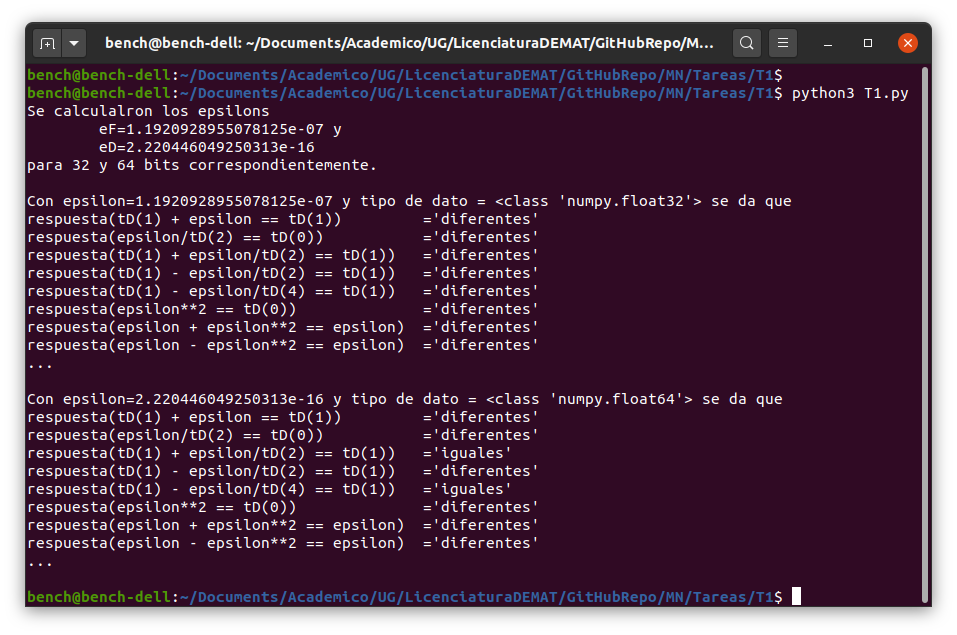
\includegraphics[scale=1.1]{assets/E2-1.png}
	\caption{Evidencia Ejecucion}
\end{figure}


    % Add a bibliography block to the postdoc
    
    
    
\end{document}
